\section{Tree-based models}

\newcommand{\treenode}[2]{
    \node[draw=black, fill=green!40, inner sep=2pt, circle] (#1) at #2 {};
}
\newcommand{\leafnode}[2]{
    \node[draw=black, inner sep=2pt] (#1) at #2 {};
}
\newsavebox{\firsttree}
\sbox{\firsttree}{
    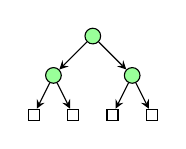
\begin{tikzpicture}
        \treenode{n0}{(0, 0)}
        \treenode{n1}{(0.5, -0.5)}
        \treenode{n2}{(-0.5, -0.5)}
        \leafnode{n3}{(0.25, -1)}
        \leafnode{n4}{(0.75, -1)}
        \leafnode{n5}{(-0.25, -1)}
        \leafnode{n6}{(-0.75, -1)}

        \draw[-stealth] (n0) -- (n1);
        \draw[-stealth] (n0) -- (n2);
        \draw[-stealth] (n1) -- (n3);
        \draw[-stealth] (n1) -- (n4);
        \draw[-stealth] (n2) -- (n5);
        \draw[-stealth] (n2) -- (n6);
    \end{tikzpicture}
}

\newsavebox{\secondtree}
\sbox{\secondtree}{
    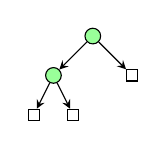
\begin{tikzpicture}
        \treenode{n0}{(0, 0)}
        \leafnode{n1}{(0.5, -0.5)}
        \treenode{n2}{(-0.5, -0.5)}
        \leafnode{n5}{(-0.25, -1)}
        \leafnode{n6}{(-0.75, -1)}

        \draw[-stealth] (n0) -- (n1);
        \draw[-stealth] (n0) -- (n2);
        \draw[-stealth] (n2) -- (n5);
        \draw[-stealth] (n2) -- (n6);
    \end{tikzpicture}
}

\newsavebox{\thirdtree}
\sbox{\thirdtree}{
    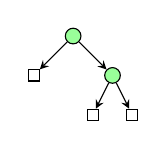
\begin{tikzpicture}
        \treenode{n0}{(0, 0)}
        \treenode{n1}{(0.5, -0.5)}
        \leafnode{n2}{(-0.5, -0.5)}
        \leafnode{n3}{(0.25, -1)}
        \leafnode{n4}{(0.75, -1)}

        \draw[-stealth] (n0) -- (n1);
        \draw[-stealth] (n0) -- (n2);
        \draw[-stealth] (n1) -- (n3);
        \draw[-stealth] (n1) -- (n4);
    \end{tikzpicture}
}

\newcommand{\treedataplot}[1]{
    \def\height{5cm}
    \def\width{8cm}

    \ifnum#1>1
        \def\width{5cm}
    \fi

    \begin{tikzpicture}
        \begin{axis}[
            height=\height,
            width=\width,
            xlabel=$x_1$,
            ylabel=$x_2$,
            zlabel=$y$,
            view={75}{10},
            x dir=reverse
        ]
            \ifnum#1<3
                \addplot3 table [
                    only marks,
                    opacity=0.5,
                    col sep=comma,
                    x=x,
                    y=y,
                    z=value
                ] {data/treedata.csv};
            \fi

            \ifnum#1>0
                \ifnum#1<2
                    \addplot3[
                        surf,
                        opacity=0.25,
                        fill=red!80!blue,
                        draw=red!80!blue,
                        domain=0:0.6, y domain=0:0.5,
                        shader=flat
                    ] {0.8};

                    \addplot3[
                        surf,
                        opacity=0.25,
                        fill=red!90!blue,
                        draw=red!90!blue,
                        domain=0:0.6, y domain=0.5:1,
                        shader=flat
                    ] {0.9};
                    \addplot3[
                        surf,
                        opacity=0.25,
                        fill=red!50!blue,
                        draw=red!50!blue,
                        domain=0.6:1, y domain=0:0.5,
                        shader=flat
                    ] {0.5};
                    \addplot3[
                        surf,
                        opacity=0.25,
                        fill=red!10!blue,
                        draw=red!10!blue,
                        domain=0.6:1, y domain=0.5:1,
                        shader=flat
                    ] {0.1};
                \fi
            \fi

            \ifnum#1>2
                \addplot3 [
                    only marks,
                    scatter,
                    scatter src=explicit,
                    point meta min=0,
                    point meta max=1,
                    colormap name=blue red
                ] table [
                    col sep=comma,
                    x=x,
                    y=y,
                    z=value,
                    meta=value
                ] {data/treedata.csv};
            \fi
        \end{axis}
    \end{tikzpicture}
}

\newcommand{\polyplot}[1]{
    \begin{tikzpicture}
        \begin{axis}[
            height=5cm,
            width=8cm,
            xlabel=$x$,
            ylabel=$y$,
            xmin=-0.1,
            xmax=1,
            xtick={-0.1, 0.175, 0.45, 0.725, 1},
            xticklabels={0, 0.25, 0.5, 0.75, 1},
            ymajorticks=false,
            ymin=-10,
            ymax=2.5,
            xtick pos=bottom
        ]
            \ifnum#1<3
                \addplot[
                    only marks,
                    blue,
                    samples=100,
                    domain=-0.1:1,
                    opacity=0.5
                ] (x, 300*x^5 - 750 * x^4 + 630 * x^3 - 210 * x^2 + 20 * x + 1 + rand);
            \fi

            \ifnum#1=1
                \addplot[
                    very thick,
                    red
                ] coordinates {
                    (-0.1,-3)
                    (-0.05, -3)
                    (-0.05, 0)
                    (0, 0)
                    (0, 1.5)
                    (0.2, 1.5)
                    (0.2, -0.5)
                    (0.65, -0.5)
                    (0.65, -1)
                    (0.7, -1)
                    (0.7, -3)
                    (0.85, -3)
                    (0.85, -6)
                    (0.95, -6)
                    (0.95, -9)
                    (1, -9)
                };
            \fi
            \ifnum#1>1
                \addplot[
                    very thick,
                    red
                ] coordinates {
                    (-0.1,-3)
                    (-0.05, -3)
                    (-0.05, 0)
                    (0, 0)
                    (0, 1)
                    (0.05, 1)
                    (0.05, 1.5)
                    (0.15, 1.5)
                    (0.15, 1)
                    (0.2, 1)
                    (0.2, 0)
                    (0.4, 0)
                    (0.4, -0.5)
                    (0.65, -0.5)
                    (0.65, -1)
                    (0.7, -1)
                    (0.7, -2.5)
                    (0.75, -2.5)
                    (0.75, -4)
                    (0.85, -4)
                    (0.85, -6)
                    (0.95, -6)
                    (0.95, -9)
                    (1, -9)
                };
            \fi
            \ifnum#1=4
                \node[anchor=south, font=\scriptsize, inner sep=2pt] at (axis cs: 0.525, -0.5) {
                    $\hat{y}=-0.5$
                };
                \draw[red] (axis cs: 0.4, 2.5) -- (axis cs: 0.4, -10);
                \draw[red] (axis cs: 0.65, 2.5) -- (axis cs: 0.65, -10);

                \node[anchor=south, font=\scriptsize, inner sep=2pt] at (axis cs: 0.3, -0.0) {
                    $\hat{y}=0.0$
                };
                \draw[red] (axis cs: 0.2, 2.5) -- (axis cs: 0.2, -10);
                \draw[red] (axis cs: 0.4, 2.5) -- (axis cs: 0.4, -10);
            \fi
        \end{axis}
    \end{tikzpicture}
}

\newsavebox{\treedata}
\sbox{\treedata}{
    \treedataplot{0}
}

\newsavebox{\treestep}
\sbox{\treestep}{
    \treedataplot{1}
}

\newsavebox{\treesquare}
\sbox{\treesquare}{
    \treedataplot{2}
}
\newsavebox{\treecolours}
\sbox{\treecolours}{
    \treedataplot{3}
}

\newsavebox{\polydata}
\sbox{\polydata}{
    \polyplot{0}
}

\newsavebox{\polystep}
\sbox{\polystep}{
    \polyplot{1}
}

\newsavebox{\polyprecise}
\sbox{\polyprecise}{
    \polyplot{2}
}
\newsavebox{\polyconstant}
\sbox{\polyconstant}{
    \polyplot{3}
}
\newsavebox{\polyregions}
\sbox{\polyregions}{
    \polyplot{4}
}

\newsavebox{\emptyplot}
\sbox{\emptyplot}{
    \begin{tikzpicture}
        \begin{axis}[
            height=5cm,
            width=8cm,
            xlabel=$x$,
            ylabel=$y$,
            ymajorticks=false,
            xmajorticks=false,
            xmin=0,
            xmax=1,
            ymin=0,
            ymax=1
        ]
            \node[] at (axis cs: 0.5, 0.5) {
                \Huge{?}
            };
        \end{axis}
    \end{tikzpicture}
}

\begin{frame}{Tree-based models: Motivation}
    \begin{tikzpicture}
        \node[] at (-5.25, -3.5) {};
        \node[] at (5.25, 3.5) {};

        \visible<1-2>{
            \node[] at (0, 1) {
                \usebox{\treedata}
            };
        }
        \visible<2>{
            \node[font=\scriptsize\selectfont] at (0, -2.5) {
                $y=
                \begin{cases}
                    0.8&x_1\leq0.6\ \&\ x_2\leq0.5\\
                    0.9&x_1\leq0.6\ \&\ x_2>0.5\\
                    0.5&x_1>0.5\ \&\ x_2\leq0.5\\
                    0.1&x_1>0.5\ \&\ x_2>0.5\\
                \end{cases}
                $
            };
        }
        \visible<3-4>{
            \node[] at (0, 1) {
                \usebox{\polydata}
            };
        }
        \visible<4>{
            \node[] at (0, -2.5) {
                $y=?x^5+?x^4+?x^3+?x^2+?x+?$
            };
        }
        \visible<5>{
            \node[] at (0, 1) {
                \usebox{\emptyplot}
            };
        }
        \visible<6>{
            \node[] at (0, 1) {
                \usebox{\treestep}
            };
        }
        \visible<7>{
            \node[] at (0, 1) {
                \usebox{\polystep}
            };
        }
        \visible<8>{
            \node[] at (0, 1) {
                \usebox{\polyprecise}
            };
        }
        \visible<9>{
            \node[] at (0, 1) {
                \usebox{\polyconstant}
            };
            \node[] at (0, -2) {
                Piecewise constant function
            };
        }
        \visible<10-11>{
            \node[] at (0, 1) {
                \usebox{\polyregions}
            };
        }
        \visible<11>{
            \node[font=\footnotesize\selectfont] at (0, -2.5) {
                $\hat{y}=
                \begin{cases}
                    ...\\
                    0.0&x\geq0.27\ \& \ x<0.45\\
                    -0.5&x\geq0.45\ \& \ x<0.69\\
                    ...\\
                \end{cases}
                $
            };
        }
    \end{tikzpicture}
\end{frame}

\newcommand{\stratificationplot}[1]{
    \begin{tikzpicture}
        \begin{axis}[
            height=4cm,
            width=4cm,
            xlabel=\scriptsize{$x_2$},
            ylabel=\scriptsize{$x_1$},
            ticklabel style={font=\scriptsize\selectfont},
            tick style={draw=none},
            clip=false,
            xmin=-0.05,
            xmax=0.95,
            ymin=-0.05,
            ymax=0.95,
            point meta min=0,
            point meta max=1,
            colormap name=blue red,
            colorbar,
            colorbar style={
                title=\scriptsize{$y$}
            }
        ]
            \addplot[
                only marks,
                scatter,
                scatter src=explicit
            ] table [
                col sep=comma,
                x=y,
                y=x,
                meta=value
            ] {data/treedata.csv};

            \ifnum#1>0
                \draw[very thick] (axis cs: -0.05, 0.55) -- (axis cs: 0.95, 0.55);
            \fi
            \ifnum#1>1
                \draw[very thick] (axis cs: 0.45, 0.55) -- (axis cs: 0.45, 0.95);
            \fi
            \ifnum#1>2
                \draw[very thick] (axis cs: 0.45, 0.55) -- (axis cs: 0.45, -0.05);
            \fi
            \ifnum#1>3
                \draw[very thick] (axis cs: -0.05, 0.75) -- (axis cs: 0.45, 0.75);
            \fi
            \ifnum#1>4
                \draw[very thick] (axis cs: 0.05, -0.05) -- (axis cs: 0.05, 0.95);
                \draw[very thick] (axis cs: 0.15, -0.05) -- (axis cs: 0.15, 0.95);
                \draw[very thick] (axis cs: 0.25, -0.05) -- (axis cs: 0.25, 0.95);
                \draw[very thick] (axis cs: 0.35, -0.05) -- (axis cs: 0.35, 0.95);
                \draw[very thick] (axis cs: 0.45, -0.05) -- (axis cs: 0.45, 0.95);
                \draw[very thick] (axis cs: 0.55, -0.05) -- (axis cs: 0.55, 0.95);
                \draw[very thick] (axis cs: 0.65, -0.05) -- (axis cs: 0.65, 0.95);
                \draw[very thick] (axis cs: 0.75, -0.05) -- (axis cs: 0.75, 0.95);
                \draw[very thick] (axis cs: 0.85, -0.05) -- (axis cs: 0.85, 0.95);

                \draw[very thick] (axis cs: -0.05, 0.05) -- (axis cs: 0.95, 0.05);
                \draw[very thick] (axis cs: -0.05, 0.15) -- (axis cs: 0.95, 0.15);
                \draw[very thick] (axis cs: -0.05, 0.25) -- (axis cs: 0.95, 0.25);
                \draw[very thick] (axis cs: -0.05, 0.35) -- (axis cs: 0.95, 0.35);
                \draw[very thick] (axis cs: -0.05, 0.45) -- (axis cs: 0.95, 0.45);
                \draw[very thick] (axis cs: -0.05, 0.55) -- (axis cs: 0.95, 0.55);
                \draw[very thick] (axis cs: -0.05, 0.65) -- (axis cs: 0.95, 0.65);
                \draw[very thick] (axis cs: -0.05, 0.75) -- (axis cs: 0.95, 0.75);
                \draw[very thick] (axis cs: -0.05, 0.85) -- (axis cs: 0.95, 0.85);
            \fi
        \end{axis}
    \end{tikzpicture}
}

\newsavebox{\stratificationpoints}
\sbox{\stratificationpoints}{
    \stratificationplot{0}
}
\newsavebox{\stratificationfirst}
\sbox{\stratificationfirst}{
    \stratificationplot{1}
}
\newsavebox{\stratificationsecond}
\sbox{\stratificationsecond}{
    \stratificationplot{2}
}
\newsavebox{\stratificationthird}
\sbox{\stratificationthird}{
    \stratificationplot{3}
}
\newsavebox{\stratificationfourth}
\sbox{\stratificationfourth}{
    \stratificationplot{4}
}
\newsavebox{\stratificationlast}
\sbox{\stratificationlast}{
    \stratificationplot{5}
}

\newcommand{\treeplot}[1]{
    \begin{tikzpicture}
        \node[] at (-1, 0.5) {};
        \node[] at (1.75, -3.5) {};

        \colorlet{pathcolour}{black}

        \ifnum#1=4
            \colorlet{pathcolour}{red}
        \fi

        \node[draw=black, font=\small\selectfont, draw=pathcolour, text=pathcolour] (n0) at (0, 0) {
            $x_1 < 0.6$
        };

        \node[font=\small\selectfont, minimum height=1cm] (n10) at (-0.75, -1.5) {};
        \node[font=\small\selectfont, minimum height=1cm] (n11) at (0.75, -1.5) {};
        \node[font=\small\selectfont, minimum height=1cm] (n20) at (0, -3) {};
        \node[font=\small\selectfont, minimum height=1cm] (n21) at (1.5, -3) {};


        \draw[-stealth] (n0) -- (n10) node [midway, left] {Yes};
        \draw[-stealth, pathcolour] (n0) -- (n11) node [midway, right, pathcolour] {No};

        \ifnum#1>0
            \node[font=\small\selectfont] (n10) at (-0.75, -1.5) {
                0.85
            };
        \fi
        \ifnum#1>1
            \node[draw=black, font=\small\selectfont, draw=pathcolour, text=pathcolour] (n11) at (0.75, -1.5) {
                $x_2 < 0.5$
            };

            \draw[-stealth, pathcolour] (n11) -- (n20) node [midway, left] {Yes};
            \draw[-stealth] (n11) -- (n21) node [midway, right] {No};
        \fi
        \ifnum#1>2
            \node[font=\small\selectfont, text=pathcolour] (n20) at (0, -3) {
                0.5
            };
            \node[font=\small\selectfont] (n21) at (1.5, -3) {
                0.1
            };
        \fi

    \end{tikzpicture}
}

\newsavebox{\treeroot}
\sbox{\treeroot}{
    \treeplot{0}
}
\newsavebox{\treeleft}
\sbox{\treeleft}{
    \treeplot{1}
}
\newsavebox{\treeright}
\sbox{\treeright}{
    \treeplot{2}
}
\newsavebox{\treefull}
\sbox{\treefull}{
    \treeplot{3}
}
\newsavebox{\treeprediction}
\sbox{\treeprediction}{
    \treeplot{4}
}

\newsavebox{\treecomplexity}
\sbox{\treecomplexity}{
    \begin{tikzpicture}
        \draw[stealth-stealth, thick] (-4, 0) -- (4, 0) node [midway, below] {Tree complexity};
        \node[circle, draw=black, fill=green!40, inner sep=2pt] (n00) at (-3.5, -0.2) {};

        \draw[-stealth] (n00) -- ($ (n00) - (0.3, 0.4) $);
        \draw[-stealth] (n00) -- ($ (n00) - (-0.3, 0.4) $);

        \node[circle, draw=black, fill=green!40, inner sep=2pt] (n10) at (3.5, -0.2) {};
        \node[circle, draw=black, fill=green!40, inner sep=2pt] (n11) at ($ (n10) - (0.3, 0.4) $) {};
        \node[circle, draw=black, fill=green!40, inner sep=2pt] (n12) at ($ (n10) - (-0.3, 0.4) $) {};

        \draw[-] (n10) -- (n11);
        \draw[-] (n10) -- (n12);

        \node[circle, draw=black, fill=green!40, inner sep=2pt] (n13) at ($ (n11) - (0.2, 0.4) $) {};
        \node[circle, draw=black, fill=green!40, inner sep=2pt] (n14) at ($ (n12) - (-0.2, 0.4) $) {};

        \draw[-stealth] (n11) -- ($ (n11) - (-0.2, 0.4) $);
        \draw[-stealth] (n12) -- ($ (n12) - (0.2, 0.4) $);
        \draw[] (n11) -- (n13);
        \draw[] (n12) -- (n14);

        \draw[-stealth] (n13) -- ($ (n13) - (0.2, 0.4) $);
        \draw[-stealth] (n13) -- ($ (n13) - (-0.2, 0.4) $);
        \draw[-stealth] (n14) -- ($ (n14) - (0.2, 0.4) $);
        \draw[-stealth] (n14) -- ($ (n14) - (-0.2, 0.4) $);

        \node[align=center] at (2.8, 0.7) {
            Overfitting\\
            High variance
        };
        \node[align=center] at (-2.8, 0.7) {
            Underfitting\\
            High bias
        };

    \end{tikzpicture}
}

\newcommand{\decisiontree}[1]{
    \begin{tikzpicture}
        \treenode{n0}{(0, 0)}
        \treenode{n1}{($ (n0) - (0.5, 0.5) $)}
        \treenode{n2}{($ (n0) - (-0.5, 0.5) $)}
        \treenode{n3}{($ (n1) - (0.25, 0.5) $)}
        \treenode{n4}{($ (n1) - (-0.25, 0.5) $)}
        \leafnode{n5}{($ (n3) - (0.125, 0.5) $)}
        \leafnode{n6}{($ (n3) - (-0.125, 0.5) $)}
        \leafnode{n7}{($ (n4) - (0.125, 0.5) $)}
        \leafnode{n8}{($ (n4) - (-0.125, 0.5) $)}
        \leafnode{n9}{($ (n2) - (0.25, 0.5) $)}
        \treenode{n10}{($ (n2) - (-0.25, 0.5) $)}
        \leafnode{n11}{($ (n10) - (0.125, 0.5) $)}

        \ifnum#1=0
            \treenode{n12}{($ (n10) - (-0.125, 0.5) $)}
            \leafnode{n13}{($ (n12) - (0.125, 0.5) $)}
            \leafnode{n14}{($ (n12) - (-0.125, 0.5) $)}

            \draw[-stealth] (n12) -- (n13);
            \draw[-stealth] (n12) -- (n14);
        \fi
        \ifnum#1=1
            \leafnode{n12}{($ (n10) - (-0.125, 0.5) $)}
        \fi

        \draw[-stealth] (n0) -- (n1);
        \draw[-stealth] (n0) -- (n2);
        \draw[-stealth] (n1) -- (n3);
        \draw[-stealth] (n1) -- (n4);
        \draw[-stealth] (n3) -- (n5);
        \draw[-stealth] (n3) -- (n6);
        \draw[-stealth] (n4) -- (n7);
        \draw[-stealth] (n4) -- (n8);
        \draw[-stealth] (n2) -- (n9);
        \draw[-stealth] (n2) -- (n10);
        \draw[-stealth] (n10) -- (n11);
        \draw[-stealth] (n10) -- (n12);
    \end{tikzpicture}
}

\newsavebox{\fulldecisiontree}
\sbox{\fulldecisiontree}{
    \decisiontree{0}
}
\newsavebox{\pruneddecisiontree}
\sbox{\pruneddecisiontree}{
    \decisiontree{1}
}

\newcommand{\pruningplot}[1]{
    \begin{tikzpicture}
        \node[] at (-4.4, 3) {};
        \node[] at (4.4, -3) {};

        \node[anchor=south west] at (-3.9, 0) {
            \usebox{\fulldecisiontree}
        };

        \ifnum#1>0
            \draw[|-stealth] (-2.6, 0) -- (4, 0) node [midway, below] {$\alpha$};
            \node[anchor=north] at (-2.6, -0.1) {$0$};
            \node[anchor=north] at (4, -0.1) {$\infty$};

            \node[align=center] at (0, -2) {
                $\sum\limits_{i=0}^n (y_i - \hat{y}_i)^2 + \alpha |T|$,\\
                $|T|$=number of leaf nodes
            };
        \fi

        \ifnum#1>1
            \node[anchor=south] at (-0.3, 0) {
                \usebox{\pruneddecisiontree}
            };
        \fi
        \ifnum#1>2
            \leafnode{empty}{(3.9, 0.22)}
            \node[anchor=south, font=\Huge\selectfont] at (2.35, 0.22) {$\ldots$};
        \fi

        \ifnum#1>3
            \node[] at (-2.6, 2.8) {$|T|=n$};
            \node[] at (-0.4, 2.8) {$|T|=n-1$};
            \node[] at (2.35, 2.8) {$\ldots$};
            \node[] at (4, 2.8) {$|T|=1$};
        \fi

    \end{tikzpicture}
}
\newsavebox{\pruningtree}
\sbox{\pruningtree}{
    \pruningplot{0}
}
\newsavebox{\pruningaxis}
\sbox{\pruningaxis}{
    \pruningplot{1}
}
\newsavebox{\pruningpruned}
\sbox{\pruningpruned}{
    \pruningplot{2}
}
\newsavebox{\pruningfull}
\sbox{\pruningfull}{
    \pruningplot{3}
}
\newsavebox{\pruningannotated}
\sbox{\pruningannotated}{
    \pruningplot{4}
}

\newsavebox{\treetradeoff}
\sbox{\treetradeoff}{
    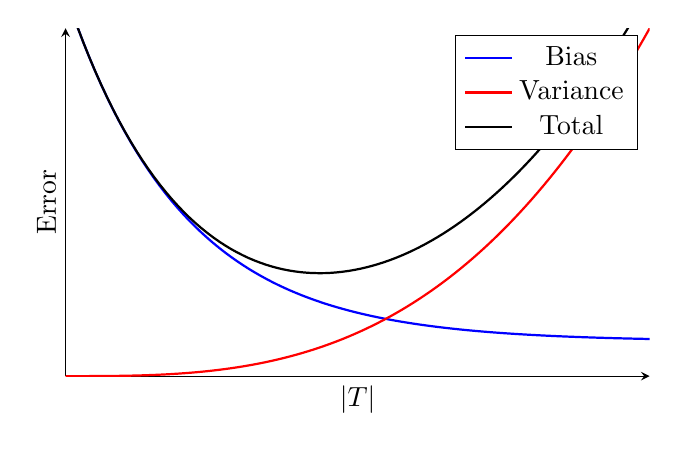
\begin{tikzpicture}
        \begin{axis}[
            height=6cm,
            width=9cm,
            xlabel={$|T|$},
            axis x line*=bottom,
            axis y line*=left,
            axis line style={-stealth},
            xmajorticks=false,
            ymajorticks=false,
            xmin=0,
            xmax=1,
            ymin=0,
            ymax=1,
            ylabel=Error
        ]
            \addplot[blue, thick, domain=0:1, samples=100] (x, {exp(-5 * x) + 0.1});
            \addplot[red, thick, domain=0:1, samples=100] (x, x^3);
            \addplot[black, thick, domain=0:1, samples=100] (x, {exp(-5 * x) + 0.1 + x^3});
            %\addplot[red, smooth, thick] (x, x^2);
            \legend{Bias, Variance, Total}


        \end{axis}
    \end{tikzpicture}
}

\begin{frame}{Tree-based models: Decision trees}
    \begin{tikzpicture}
        \node[] at (-5.25, -3.5) {};
        \node[] at (5.25, 3.5) {};

        \visible<1>{
            \node[anchor=west, inner sep=-7pt] at (-5.25, 0) {
                \usebox{\treesquare}
            };
        }
        \visible<2>{
            \node[anchor=west, inner sep=-7pt] at (-5.25, 0) {
                \usebox{\treecolours}
            };
        }
        \visible<2-3,8-13>{
            \node[anchor=east] at (5.25, 0.3) {
                \usebox{\stratificationpoints}
            };
        }
        \visible<4>{
            \node[anchor=north] at (-3, 2.5) {
                \usebox{\treeroot}
            };
        }
        \visible<4-5,13-16>{
            \node[anchor=east] at (5.25, 0.3) {
                \usebox{\stratificationfirst}
            };
        }
        \visible<5>{
            \node[anchor=north] at (-3, 2.5) {
                \usebox{\treeleft}
            };
        }
        \visible<6>{
            \node[anchor=north] at (-3, 2.5) {
                \usebox{\treeright}
            };
        }
        \visible<6-7>{
            \node[anchor=east] at (5.25, 0.3) {
                \usebox{\stratificationsecond}
            };
        }
        \visible<7>{
            \node[anchor=north] at (-3, 2.5) {
                \usebox{\treefull}
            };
        }
        \visible<9-12>{
            \node[] (predictor) at (-3, 0.5) {
                $x_1$ or $x_2$?
            };
        }
        \visible<10-12>{
            \node[font=\footnotesize] (x1) at (-4, -0.5) {
                [0, \ldots, 0.6, \ldots, 0.9]
            };
            \node[font=\footnotesize] (x2) at (-2, -0.5) {
                [0, 0.1, \ldots, 0.9]
            };
            \draw[-stealth] ($ (predictor.south) - (0.7, 0) $) -- (x1);
            \draw[-stealth] ($ (predictor.south) + (0.6, 0) $) -- (x2);
        }
        \visible<11>{
            \node[font=\footnotesize, inner sep=2pt] (l2) at ($ (x1.south) - (0.1, 0.5) $) {
                $\ell_1$
            };
            \draw[-stealth] ($ (l2) + (0, 0.55) $) -- (l2);
        }
        \visible<12>{
            \node[font=\footnotesize, inner sep=2pt, red] (l2) at ($ (x1.south) - (0.1, 0.5) $) {
                $\ell_1$
            };
            \draw[-stealth, red] ($ (l2) + (0, 0.55) $) -- (l2);
        }
        \visible<11-12>{
            \node[font=\footnotesize, inner sep=2pt] (l1) at ($ (x1.south) - (0.66, 0.5) $) {
                $\ell_0$
            };
            \draw[-stealth] ($ (l1) + (0, 0.55) $) -- (l1);
            \node[font=\footnotesize, inner sep=2pt] (l3) at ($ (x1.south) - (-0.66, 0.5) $) {
                $\ell_2$
            };
            \draw[-stealth] ($ (l3) + (0, 0.55) $) -- (l3);

            \node[font=\footnotesize, inner sep=2pt] (l4) at ($ (x2.south) - (0.66, 0.5) $) {
                $\ell_3$
            };
            \draw[-stealth] ($ (l4) + (0, 0.55) $) -- (l4);
            \node[font=\footnotesize, inner sep=2pt] (l5) at ($ (x2.south) - (0.23, 0.5) $) {
                $\ell_4$
            };
            \draw[-stealth] ($ (l5) + (0, 0.55) $) -- (l5);
            \node[font=\footnotesize, inner sep=2pt] (l6) at ($ (x2.south) - (-0.66, 0.5) $) {
                $\ell_5$
            };
            \draw[-stealth] ($ (l6) + (0, 0.55) $) -- (l6);
        }
        \visible<13-16>{
            \node[anchor=north] at (-2.2, 1.5) {
                \usebox{\treeroot}
            };
        }
        \visible<14-16>{
            \node[] (right) at (-1.35, -0.8) {
                $x_1$ or $x_2$?
            };
            \node[] (left) at (-3.55, -0.8) {
                $x_1$ or $x_2$?
            };

            \node[font=\footnotesize] (left1) at ($ (left) - (1.1, 1) $) {
                [0, \ldots, 0.5]
            };
            \node[font=\footnotesize] (left2) at ($ (left) - (-0.3, 1) $) {
                [0, \ldots, 0.9]
            };

            \node[font=\footnotesize] (right1) at ($ (right) - (0.3, 1) $) {
                [0.6, \ldots, 0.9]
            };
            \node[font=\footnotesize] (right2) at ($ (right) - (-1.1, 1) $) {
                [0, \ldots, 0.9]
            };
            \draw[-stealth] (right) -- (right1);
            \draw[-stealth] (right) -- (right2);
            \draw[-stealth] (left) -- (left1);
            \draw[-stealth] (left) -- (left2);
        }
        \visible<15-16>{
            \draw[thick, dashed] (-2.5, -0.5) -- (-2.5, -2.5);
        }
        \visible<14-15>{
            \node[font=\footnotesize] (left1) at ($ (left) - (1.1, 1) $) {
                [0, \ldots, 0.5]
            };

            \node[font=\footnotesize] (right1) at ($ (right) - (0.3, 1) $) {
                [0.6, \ldots, 0.9]
            };
        }
        \visible<16>{
            \node[font=\footnotesize] (left1) at ($ (left) - (1.1, 1) $) {
                [0, \ldots, {\color{red}0.5}]
            };

            \node[font=\footnotesize] (right1) at ($ (right) - (0.3, 1) $) {
                [{\color{red}0.6}, \ldots, 0.9]
            };
        }
        \visible<17-18>{
            \node[anchor=north] at (0, 2.5) {
                \usebox{\treefull}
            };
        }
        \visible<18-20>{
            \node[red] at (-0.35, 2.7) {
                $x=(0.8, 0.3)$
            };
        }
        \visible<19-20>{
            \node[anchor=north] at (0, 2.5) {
                \usebox{\treeprediction}
            };
        }
        \visible<20>{
            \node[align=center] at (0, -2.5) {
                Why was $\hat{y}=0.5$?\\Because $x_1\geq0.6$ and $x_2 < 0.5$.
            };
        }
        \visible<21>{
            \node[] at (0, 0) {
                \usebox{\stratificationpoints}
            };
        }
        \visible<22>{
            \node[] at (0, 0) {
                \usebox{\stratificationfirst}
            };
        }
        \visible<23>{
            \node[] at (0, 0) {
                \usebox{\stratificationsecond}
            };
        }
        \visible<24>{
            \node[] at (0, 0) {
                \usebox{\stratificationthird}
            };
        }
        \visible<25>{
            \node[] at (0, 0) {
                \usebox{\stratificationfourth}
            };
        }
        \visible<26>{
            \node[] at (0, 0) {
                \usebox{\stratificationlast}
            };
        }
        \visible<27-29>{
            \node[] at (0, 0) {
                \usebox{\stratificationsecond}
            };
        }
        \visible<28>{
            \node[font=\Large\selectfont\bfseries] at (0, 0.25) {
                x
            };
            \node[] at (0, -2.5) {
                $\hat{y}=0.8$
            };
        }
        \visible<29>{
            \node[font=\Large\selectfont\bfseries] at (0, 0.45) {
                x
            };
            \node[] at (0, -2.5) {
                $\hat{y}=0.1$
            };
        }
        \visible<30>{
            \node[] at (0, 0) {
                \usebox{\treecomplexity}
            };
        }
        \visible<31-37>{
            \node[draw=black] (root) at (0, 1) {
                $x_1 < a$
            };
            \node[] (n1) at (1, 0) {
                $x_1$ or $x_2$?
            };
            \node[font=\footnotesize\selectfont] (t1) at (0.1, -1) {
                $[t_0,\ldots,t_{n-1}]$
            };
            \node[font=\footnotesize\selectfont] (t2) at (1.9, -1) {
                $[t_0,\ldots,t_{n-1}]$
            };

            \draw[-stealth] (root) -- (n1);
            \draw[-stealth] ($ (n1.south) - (0.6, 0) $) -- (t1);
            \draw[-stealth] ($ (n1.south) + (0.6, 0) $) -- (t2);
        }
        \visible<32-37>{
            \node[anchor=south] at (0, 1.3) {
                $\vdots$
            };
            \node[font=\fontsize{34}{34}\selectfont, anchor=south east, text=red] (parenthesis) at ($ (root.south west) - (0, 0.2) $) {
                \{
            };
            \node[align=right, text=red, anchor=east] at (parenthesis.west) {
                tree: $t$\\
                depth: $d-1$
            };
        }
        \visible<33-37>{
            \node[font=\fontsize{34}{34}\selectfont, anchor=south east, text=red] (parenthesis2) at ($ (root.south west) + (0, -2) $) {
                \{
            };
            \node[align=right, text=red, anchor=east] at (parenthesis2.west) {
                node: $n$\\
                depth: $d$
            };
        }
        \visible<34>{
            \node[align=left, font=\small\linespread{0.9}\selectfont, draw=black, fill=white] at (-2.5, -2.5) {
                if $d>max\_depth$:\\
                \ \ \ \ stop\\
                else:\\
                \ \ \ \ continue
            };
        }
        \visible<35-37>{
            \node[font=\small] (l0) at ($ (t1) - (0.6, 1) $) {
                $\ell_0$
            };
            \node[] (l1) at ($ (t1) - (-0.6, 1) $) {
                $\ell_1$
            };
            \node[font=\small] (l2) at ($ (t2) - (0.6, 1) $) {
                $\ell_1$
            };
            \node[] (l3) at ($ (t2) - (-0.6, 1) $) {
                $\ell_2$
            };
            \draw[-stealth] ($ (l0) + (0, 0.7) $) -- (l0);
            \draw[-stealth] ($ (l1) + (0, 0.7) $) -- (l1);
            \draw[-stealth] ($ (l2) + (0, 0.7) $) -- (l2);
            \draw[-stealth] ($ (l3) + (0, 0.7) $) -- (l3);

            \node[] at ($ (n1.south) - (0, 2.3) $) {
                $\ell^{d}=\min{(\ell)}$
            };
        }
        \visible<36-37>{
            \node[text=red] (ell) at ($ (root.north east) + (1.5, 0) $) {
                $\ell^{d-1}$
            };
            \draw[red!50, line width=5pt, -stealth] ($ (ell.west) - (0.8, 0) $) -- (ell.west);
        }
        \visible<37>{
            \node[align=left, font=\small\linespread{0.9}\selectfont, draw=black, fill=white] at (-2.5, -2.5) {
                if $(\ell^{d-1}-\ell^{d}) < t$:\\
                \ \ \ \ stop\\
                else:\\
                \ \ \ \ continue
            };
        }
        \visible<38>{
            \node[font=\tiny\selectfont] at (0, 0) {
                \url{https://scikit-learn.org/dev/modules/generated/sklearn.tree.DecisionTreeClassifier.html}
            };
        }
        \visible<39>{
            \node[] at (0, 0) {
                \usebox{\pruningtree}
            };
        }
        \visible<40>{
            \node[] at (0, 0) {
                \usebox{\pruningaxis}
            };
        }
        \visible<41>{
            \node[] at (0, 0) {
                \usebox{\pruningpruned}
            };
        }
        \visible<42>{
            \node[] at (0, 0) {
                \usebox{\pruningfull}
            };
        }
        \visible<43>{
            \node[] at (0, 0) {
                \usebox{\pruningannotated}
            };
        }
        \visible<44>{
            \node[] at (0, 0) {
                \usebox{\treetradeoff}
            };
        }
        \visible<45>{
            \node[text width=10cm] at (0, 0) {
                \underline{Decision trees}: Segments the feature space into regions via the application of multiple binary splits.
                \begin{itemize}
                    \item Can be used for classification and regression
                    \item[\textcolor{green}{+}] Very interpretable
                    \item[\textcolor{red}{-}] Quite bad
                    \begin{itemize}
                        \item Prone to overfitting
                        \item Small changes in $x$ can yield large differences in $\hat{y}$
                    \end{itemize}
                    \item Complexity can be controlled via limiting tree size during fitting
                    \item Can be pruned afterwards to determine optimal size
                \end{itemize}
            };
        }

    \end{tikzpicture}
\end{frame}

\newcommand{\datasetnode}[3]{
    \node[fill=#3, draw=black, minimum width=0.4cm, minimum height=0.6cm, inner sep=0pt, font=\scriptsize\selectfont] at #1 {#2};
}

\newsavebox{\firstdataset}
\sbox{\firstdataset}{
    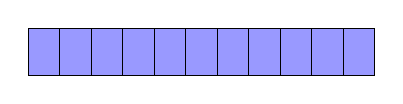
\begin{tikzpicture}
        \datasetnode{(0, 0)}{}{blue!40};
        \datasetnode{(0.4, 0)}{}{blue!40};
        \datasetnode{(0.8, 0)}{}{blue!40};
        \datasetnode{(1.2, 0)}{}{blue!40};
        \datasetnode{(1.6, 0)}{}{blue!40};
        \datasetnode{(2.0, 0)}{}{blue!40};
        \datasetnode{(2.4, 0)}{}{blue!40};
        \datasetnode{(2.8, 0)}{}{blue!40};
        \datasetnode{(3.2, 0)}{}{blue!40};
        \datasetnode{(3.6, 0)}{}{blue!40};
        \datasetnode{(4, 0)}{}{blue!40};
    \end{tikzpicture}
}

\newsavebox{\seconddataset}
\sbox{\seconddataset}{
    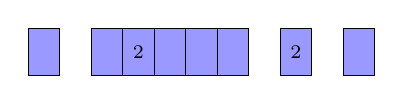
\begin{tikzpicture}
        \datasetnode{(0, 0)}{}{blue!40};
        \datasetnode{(0.8, 0)}{}{blue!40};
        \datasetnode{(1.2, 0)}{2}{blue!40};
        \datasetnode{(1.6, 0)}{}{blue!40};
        \datasetnode{(2.0, 0)}{}{blue!40};
        \datasetnode{(2.4, 0)}{}{blue!40};
        \datasetnode{(3.2, 0)}{2}{blue!40};
        \datasetnode{(4, 0)}{}{blue!40};
    \end{tikzpicture}
}

\newsavebox{\thirddataset}
\sbox{\thirddataset}{
    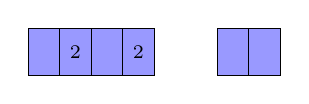
\begin{tikzpicture}
        \datasetnode{(0.4, 0)}{}{blue!40};
        \datasetnode{(0.8, 0)}{2}{blue!40};
        \datasetnode{(1.2, 0)}{}{blue!40};
        \datasetnode{(1.6, 0)}{2}{blue!40};
        \datasetnode{(2.8, 0)}{}{blue!40};
        \datasetnode{(3.2, 0)}{}{blue!40};
    \end{tikzpicture}
}

\begin{frame}{Tree-based methods: Ensembles}
    \begin{tikzpicture}
        \node[] at (-5.25, -3.5) {};
        \node[] at (5.25, 3.5) {};

        \visible<1-2>{
            \node[] at (-2, 0) {
                \usebox{\firsttree}
            };
            \draw[-stealth, line width=5pt, gray!50] (-1, 0) -- (1.2, 0);
        }
        \visible<1>{
            \node[font=\Huge\selectfont] at (2, 0) {
                \emoji{woozy-face}
            };
        }
        \visible<2>{
            \node[font=\Huge\selectfont] (face) at (2, 0) {
                \emoji{relieved-face}
            };
            \node[] at (-1, 1.5) {
                \usebox{\firsttree}
            };
            \node[] at (-1, -1.5) {
                \usebox{\firsttree}
            };
            \draw[-stealth, line width=5pt, gray!50] (0, 1.2) -- (face) ;
            \draw[-stealth, line width=5pt, gray!50] (0, -1.2) -- (face) ;
        }
        \visible<3>{
            \node[text width=10cm] at (0, 0) {
                \underline{Ensembling}: Combining multiple weak learners can improve performance.
                \begin{itemize}
                    \item A single prediction is achieved by averaging or majority voting
                    \item Models should ideally be diverse
                \end{itemize}
            };
        }
        \visible<4-8>{
            \node[label=below:\scriptsize{Dataset}, inner sep=2pt] (data) at (-2, 0) {
                \usebox{\firstdataset}
            };
        }
        \visible<5-6,8>{
            \node[] at (3, 0) {
                \usebox{\firsttree}
            };
            \draw[-stealth, line width=5pt, gray!50] (0.5, 0) -- (2, 0);
        }
        \visible<6>{
            \node[] at (3, 1.5) {
                \usebox{\firsttree}
            };
            \node[] at (3, -1.5) {
                \usebox{\firsttree}
            };
            \draw[-stealth, line width=5pt, gray!50] (0.5, 0) -- (2, 1.2);
            \draw[-stealth, line width=5pt, gray!50] (0.5, 0) -- (2, -1.2);
        }
        \visible<7-8>{
            \node[] at (-2, 1.5) {
                \usebox{\seconddataset}
            };
            \node[] at (-2, -1.5) {
                \usebox{\thirddataset}
            };
        }
        \visible<8>{
            \node[] at (3, 1.5) {
                \usebox{\secondtree}
            };
            \node[] at (3, -1.5) {
                \usebox{\thirdtree}
            };

            \draw[-stealth, line width=5pt, gray!50] (0.5, 1.5) -- (2, 1.5);
            \draw[-stealth, line width=5pt, gray!50] (0.5, -1.5) -- (2, -1.5);
        }
        \visible<9>{
            \node[text width=10cm] at (0, 0) {
                \underline{Bootstrap aggregation (bagging)}: Create a set of datasets by sampling with replacement, and train individual models on each.
            };
        }
        \visible<10-16>{
            \node[] at (0, 1) {
                \begin{tabular}{|c|c|c|c|c|c|c|}
                    \hline
                    $\mathbf{x_1}$ & $\mathbf{x_2}$ & $\mathbf{x_3}$ & $\mathbf{x_4}$ & $\mathbf{x_5}$ & $\mathbf{x_6}$ & $\mathbf{y}$ \\
                    \hline
                    \alert<11,12,14>{0.1}&\alert<11,12,16>{0.7}&\alert<11,12,14>{0.3}&\alert<11,12,16>{0.2}&\alert<11,12,15>{0.8}&\alert<11,12,15>{0.4}&\alert<11,12,14-16>{0.5}\\
                    \alert<13,14>{0.4}&\alert<13,16>{0.5}&\alert<13,14>{0.9}&\alert<13,16>{0.3}&\alert<13,15>{0.8}&\alert<13,15>{0.2}&\alert<13,14-16>{0.6}\\
                    \alert<11,14>{0.2}&\alert<11,16>{0.3}&\alert<11,14>{0.8}&\alert<11,16>{0.1}&\alert<11,15>{0.7}&\alert<11,15>{0.5}&\alert<11,14-16>{0.7}\\
                    \alert<12,13,14>{0.3}&\alert<12,13,16>{0.6}&\alert<12,13,14>{0.2}&\alert<12,13,16>{0.4}&\alert<12,13,15>{0.9}&\alert<12,13,15>{0.1}&\alert<12,13,14-16>{0.8}\\
                    \alert<12,14>{0.5}&\alert<12,16>{0.8}&\alert<12,14>{0.1}&\alert<12,16>{0.6}&\alert<12,15>{0.2}&\alert<12,15>{0.3}&\alert<12,14-16>{0.9}\\
                    \alert<11,13,14>{0.6}&\alert<11,13,16>{0.9}&\alert<11,13,14>{0.7}&\alert<11,13,16>{0.5}&\alert<11,13,15>{0.1}&\alert<11,13,15>{0.4}&\alert<11,13,14-16>{0.8}\\
                    \hline
                \end{tabular}
            };
        }
        \visible<11-13>{
            \matrix [
                matrix of nodes,
                ampersand replacement=\&,
                nodes={
                    draw=orange,
                    fill=orange!70
                },
                nodes in empty cells
            ] at (-2.75, -2.25) {
              \& \& \& \& \& \& \\
              \& \& \& \& \& \& \\
              \& \& \& \& \& \& \\
            };
        }

        \visible<12-13>{
            \matrix [
                matrix of nodes,
                ampersand replacement=\&,
                nodes={
                    draw=orange,
                    fill=orange!50
                },
                nodes in empty cells
            ] at (0, -2.25) {
              \& \& \& \& \& \& \\
              \& \& \& \& \& \& \\
              \& \& \& \& \& \& \\
            };
        }
        \visible<13>{
            \matrix [
                matrix of nodes,
                ampersand replacement=\&,
                nodes={
                    draw=orange,
                    fill=orange!30
                },
                nodes in empty cells
            ] at (2.75, -2.25) {
              \& \& \& \& \& \& \\
              \& \& \& \& \& \& \\
              \& \& \& \& \& \& \\
            };
        }
        \visible<14-17>{
            \matrix [
                matrix of nodes,
                ampersand replacement=\&,
                nodes={
                    draw=orange,
                    fill=orange!70
                },
                nodes in empty cells
            ] at (-2.75, -2.25) {
              \& \& \\
              \& \& \\
              \& \& \\
              \& \& \\
              \& \& \\
              \& \& \\
            };
        }
        \visible<15-17>{
            \matrix [
                matrix of nodes,
                ampersand replacement=\&,
                nodes={
                    draw=orange,
                    fill=orange!50
                },
                nodes in empty cells
            ] at (0, -2.25) {
              \& \& \\
              \& \& \\
              \& \& \\
              \& \& \\
              \& \& \\
              \& \& \\
            };
        }
        \visible<16-17>{
            \matrix [
                matrix of nodes,
                ampersand replacement=\&,
                nodes={
                    draw=orange,
                    fill=orange!30
                },
                nodes in empty cells
            ] at (2.75, -2.25) {
              \& \& \\
              \& \& \\
              \& \& \\
              \& \& \\
              \& \& \\
              \& \& \\
            };
        }
        \visible<17>{
            \node[] at (-2.75, 1) {
                \usebox{\firsttree}
            };
            \draw[-stealth, line width=5pt, gray!50] (-2.75, -1) -- (-2.75, 0.25);

            \node[] at (0, 1) {
                \usebox{\secondtree}
            };
            \draw[-stealth, line width=5pt, gray!50] (0, -1) -- (0, 0.25);

            \node[] at (2.75, 1) {
                \usebox{\thirdtree}
            };
            \draw[-stealth, line width=5pt, gray!50] (2.75, -1) -- (2.75, 0.25);
        }
        \visible<18>{
            \node[text width=10cm] at (0, 0) {
                \underline{Random forests}: Fits multiple decision trees on random subsets of \textbf{both} predictors and observations.
                \begin{itemize}
                    \item Produces more diverse models than bagging
                    \item The number of predictors per tree are usually $\approx \sqrt{p}$
                    \item Requires us to select the number of trees. More trees $\rightarrow$ better performance ($\approx$ same bias, less variance)
                \end{itemize}
            };
        }
    \end{tikzpicture}
\end{frame}

\begin{frame}{Tree-based methods: Boosting}
    \begin{tikzpicture}
        \node[] at (-5.25, -3.5) {};
        \node[] at (5.25, 3.5) {};

        \visible<1>{
            \node[] at (0, 0) {
                \url{https://kaggle.com}
            };
        }
        \visible<2>{
            \node[inner sep=0pt, draw=black] at (0, 2) {
                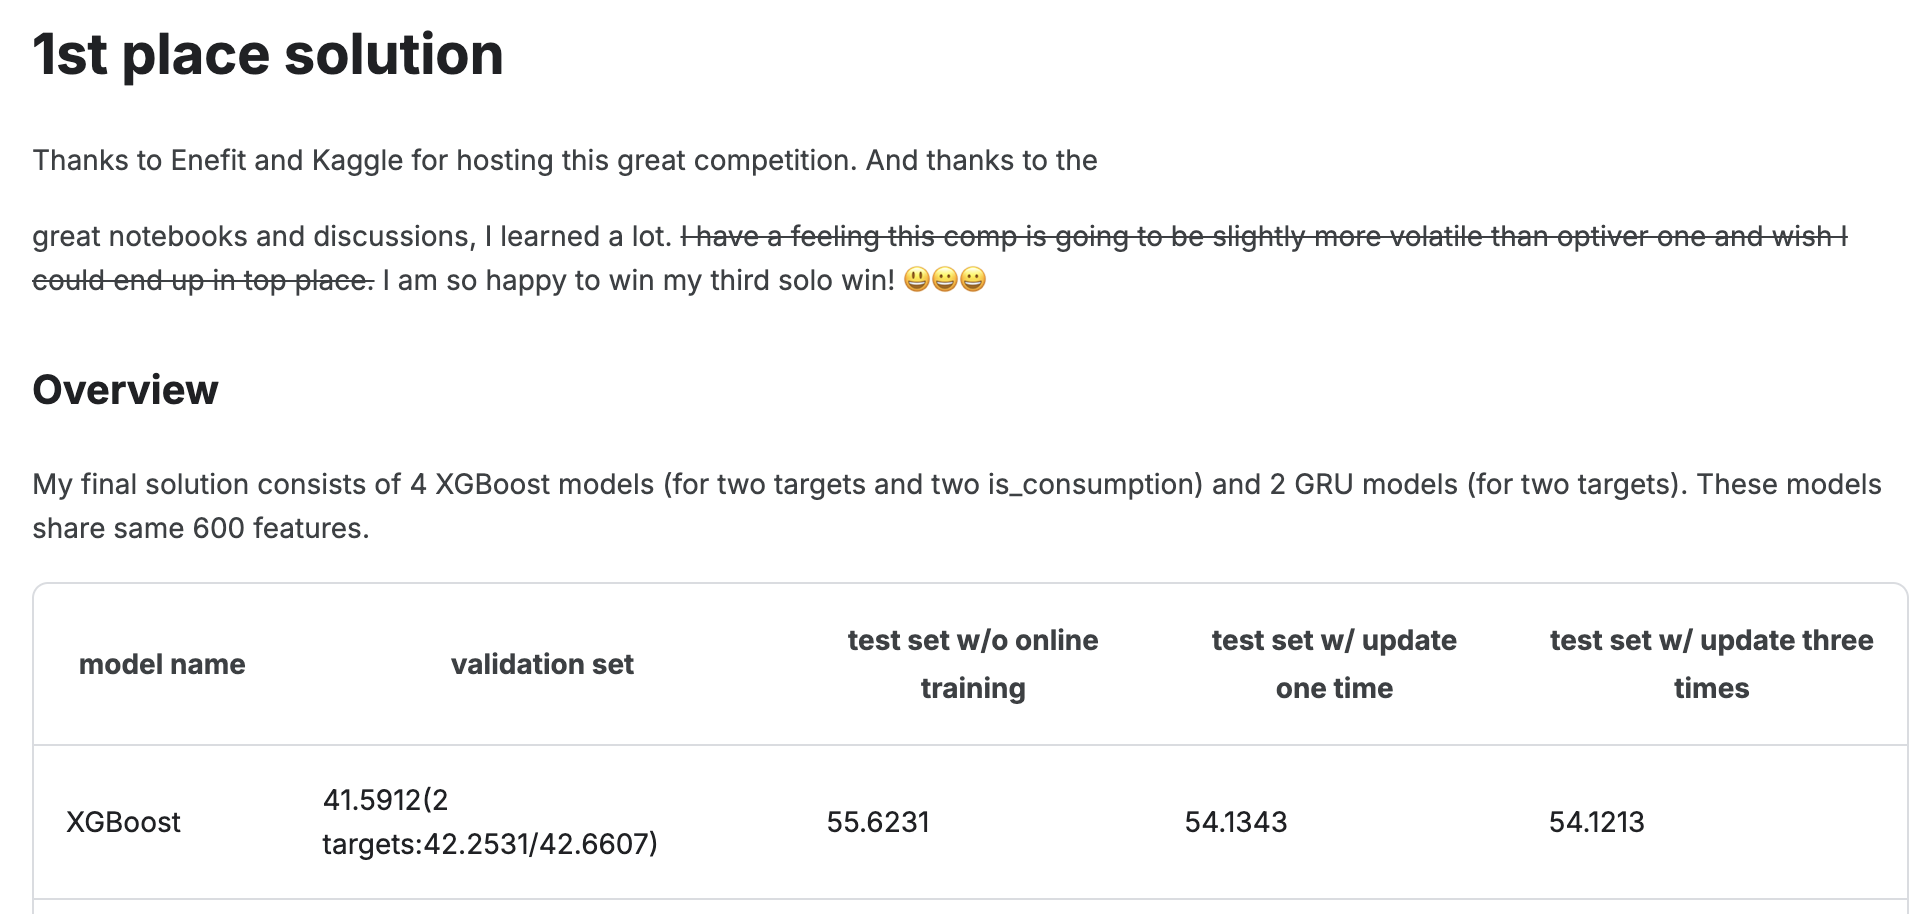
\includegraphics[width=6cm]{data/boost2.png}
            };
            \node[inner sep=0pt, draw=black] at (-2.6, -1.5) {
                
\includegraphics[width=4.5cm]{data/boost1.png}
            };
            \node[inner sep=0pt, draw=black] at (2.6, -1.5) {
                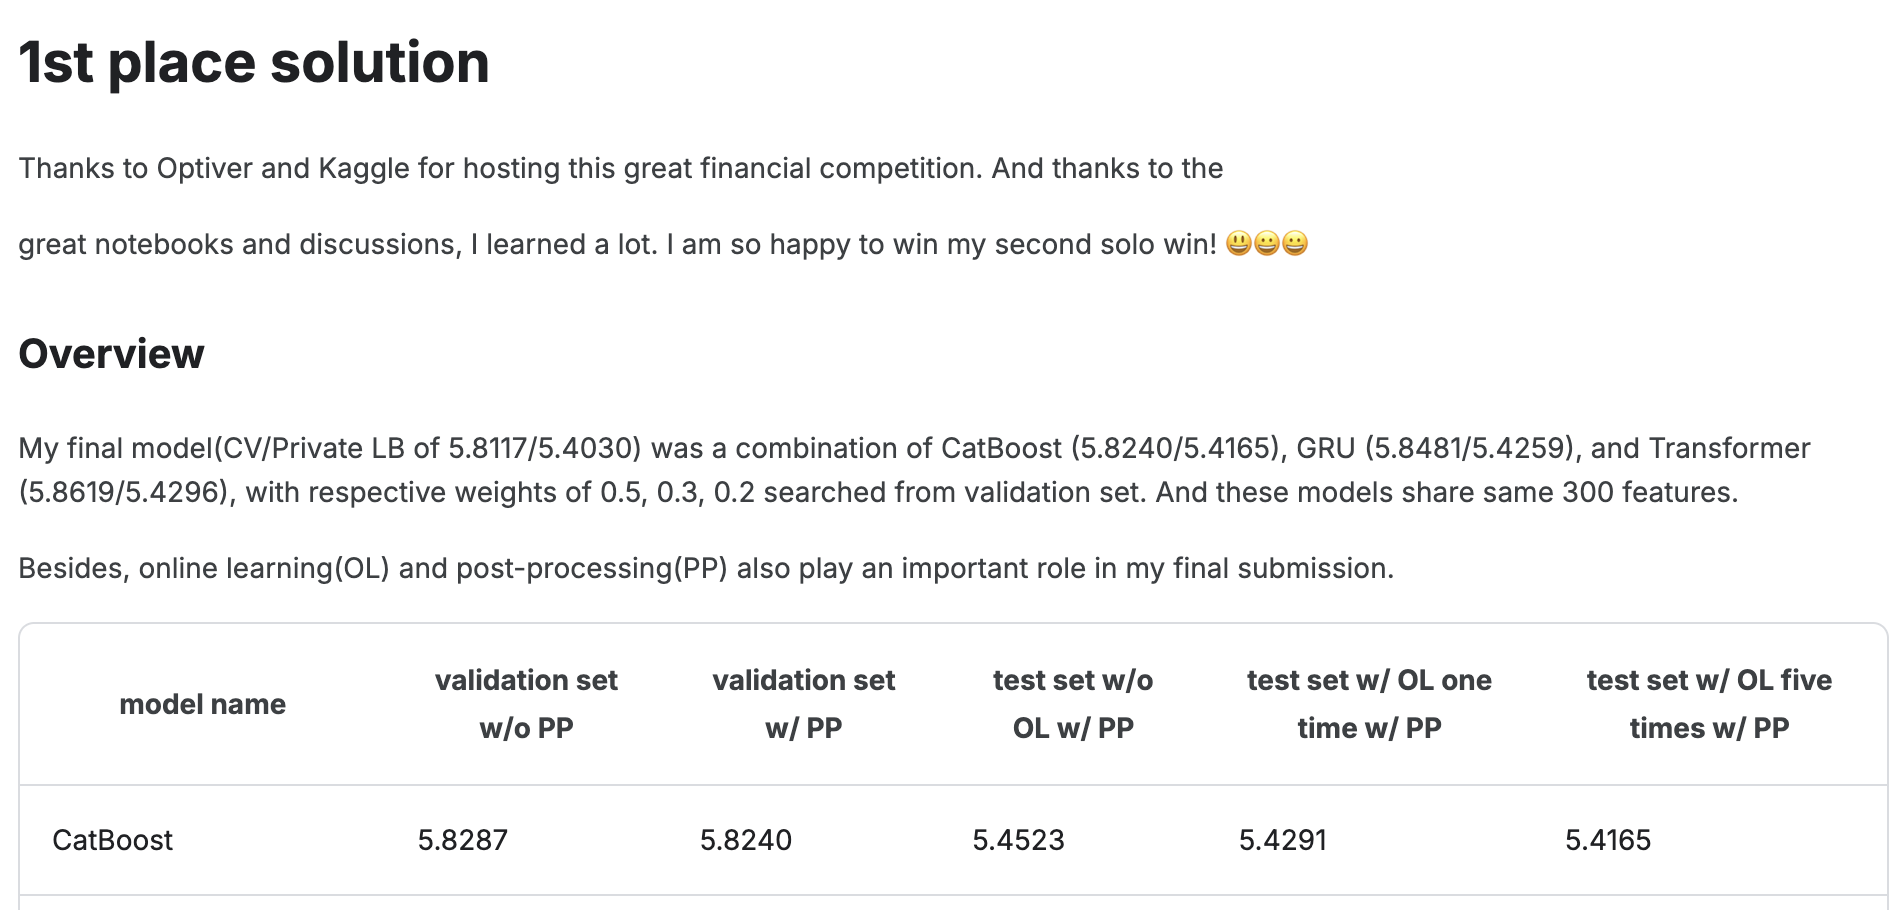
\includegraphics[width=5cm]{data/boost3.png}
            };
        }
        \visible<3>{
            \node[inner sep=0pt, draw=black] (paper) at (0, 0) {
                
\includegraphics[width=5cm]{data/paper.png}
            };
            \node[anchor=north, font=\tiny\selectfont, text width=10cm, align=center] at (paper.south) {
                Self-Attention Between Datapoints: Going Beyond
Individual Input-Output Pairs in Deep Learning, Kossen et al., preprint at arXiv, 2022
            };
        }
        \visible<4-11>{
            \node[] at (-3, 0) {
                \usebox{\firsttree}
            };
            \node[font=\tiny\selectfont] at (-3, -2) {
                $\displaystyle f_0: \min_f \sum (y_i-f(x_i))^2$
            };
        }
        \visible<5-7,9-11>{
            \node[] at (0, 0) {
                \usebox{\secondtree}
            };
        }
        \visible<5-7>{
            \node[font=\tiny\selectfont] at (0, -2) {
                $\displaystyle f_1: \min_f \sum (y_i-f(x_i))^2$
            };
        }
        \visible<6-7,10-11>{
            \node[] at (3, 0) {
                \usebox{\thirdtree}
            };
        }
        \visible<6-7>{
            \node[font=\tiny\selectfont] at (3, -2) {
                $\displaystyle f_2: \min_f \sum (y_i-f(x_i))^2$
            };
        }
        \visible<7>{
            \node[font=\footnotesize\selectfont] at (0, -3) {
                $\hat{y}=\dfrac{1}{3}\sum\limits_{i=0}^3 f_i(x)$
            };
        }
        \visible<8-11>{
            \node[font=\tiny] at (-3, -2.5) {
                $\hat{f}(x)=\lambda f_0(x)$
            };
            \node[font=\tiny] at (-3, -3) {
                $y*=y-(\hat{f}(x))$
            };
        }
        \visible<9-11>{
            \node[font=\tiny\selectfont] at (0, -2) {
                $\displaystyle f_1: \min_f \sum (y*_i-f(x_i))^2$
            };
            \node[font=\tiny] at (0, -2.5) {
                $\hat{f}(x)=\lambda (f_0(x) + f_1(x))$
            };
            \node[font=\tiny] at (0, -3) {
                $y*=y-(\hat{f}(x))$
            };
        }
        \visible<10-11>{
            \node[font=\tiny\selectfont] at (3, -2) {
                $\displaystyle f_2: \min_f \sum (y*_i-f(x_i))^2$
            };
            \node[font=\tiny] at (3, -2.5) {
                $\hat{f}(x)=\lambda (f_0(x) + f_1(x) + f_2(x))$
            };
            \node[font=\tiny] at (3, -3) {
                $y*=y-(\hat{f}(x))$
            };
        }
        \visible<12>{
            \node[text width=10cm] at (0, 0) {
                \underline{Boosting}: Fits a sequence of trees $t_0,\ldots,t_n$. Each tree $t_i$ tried to predict the residual of the preceeding model, e.g. finding the signal that the model so far has missed.
                \begin{itemize}
                    \item Works \textit{really} well
                \end{itemize}
            };
        }
        \visible<13>{
            \node[font=\fontsize{5}{5}\selectfont] at (0, 0) {
                \url{https://xgboost.readthedocs.io/en/stable/parameter.html\#parameters-for-tree-booster}
            };
        }
        \visible<14>{
            \node[font=\tiny\selectfont] at (0, 0) {
                \url{https://xgboost.readthedocs.io/en/latest/python/examples/cross_validation.html}
            };
        }
        \visible<15>{
            \node[inner sep=0pt, draw=black] at (0, 1.5) {
                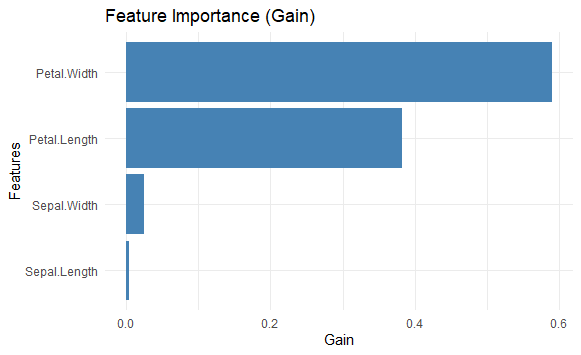
\includegraphics[width=6cm]{data/feature_importance.png}
            };
            \node[font=\fontsize{5}{5}\selectfont] at (0, -2) {
                \url{https://xgboost.readthedocs.io/en/stable/python/python_api.html\#module-xgboost.plotting}
            };
        }

    \end{tikzpicture}
\end{frame}
